  
\begin{figure}
  \centering
  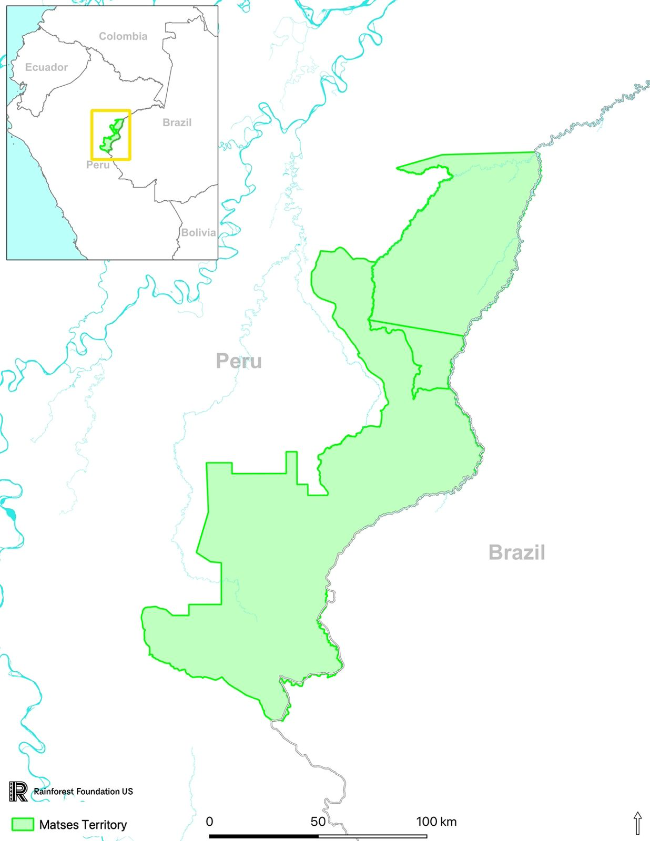
\includegraphics[width=0.9\columnwidth]{images/image13.png}
  \caption{The Matses territory --- an expansive area of nearly four million acres.}
  \label{fig:matses_territory}
\end{figure}

\begin{figure}
  \centering
  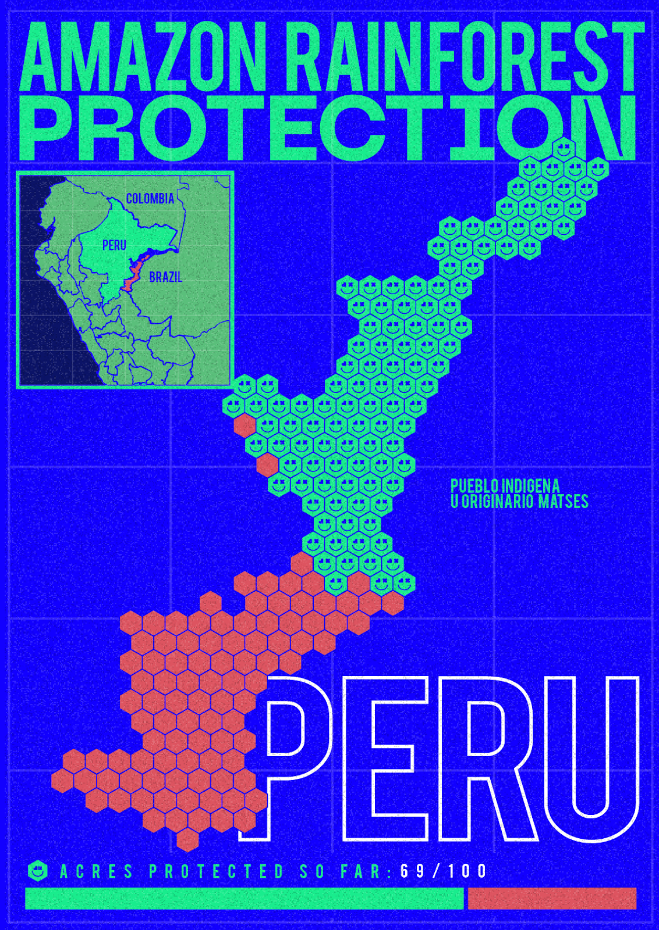
\includegraphics[width=0.9\columnwidth]{images/image14.png}
  \caption{The Matses territory rendered as a live in-platform map in Basejump}
  \label{fig:matses_map}
\end{figure}

\section{Real World Action}

A percentage of fees earned from the minting of hyperobjects will protect a real-world area of rainforest. Working in partnership with Rainforest Foundation US\footnote{Rainforest Foundation US (RFUS) is a non-profit organization that works directly with indigenous communities to protect rainforests and secure their land rights. Since 1989, RFUS has helped indigenous communities protect over 33 million acres of rainforest across Central and South America through a combination of land titling, sustainable development, and technology-enabled monitoring.}, Basejump aims to protect nearly four million acres of Peruvian rainforest with the ACTION launch.

A portion of fees may be directed towards ecosystem grants, supporting real-world impact initiatives as voted on by the community, including support for Rainforest Foundation US' work safeguarding the Matses territory---an expansive area of around four million acres, as shown in Figure \ref{fig:matses_territory}.

Proceeds will be used to implement conservation and monitoring efforts, including the construction of small guard posts along key river tributaries\footnote{The guard post monitoring system combines traditional indigenous knowledge with modern technology. Local Matses community members staff strategically placed posts equipped with solar-powered communication systems, GPS units, and drones. This enables real-time monitoring of illegal activities while providing sustainable employment for indigenous communities \cite{RFUS2024}.}. These guard posts will help Matses communities monitor and regulate entry into their lands. Once the Matses territory is fully funded, we plan to expand our work with RFUS to additional regions.

As Action users create virtual worlds, we plan to scale efforts to protect the real world. By connecting gaming communities to real-world pieces of territory they can impact, Action is offering a new onchain, gamified framework for loose-knit communities to organize in new ways and solve complex problems, outside of (but working with) centralized organizations.

Non-profit organizations that allow donors to ``adopt'' a pet, project, or cause often yield better results in terms of donor engagement, retention, and emotional satisfaction. These programs often create a stronger emotional connection between the donor and the cause. Studies show that when donors feel a personal connection to a specific beneficiary (e.g., a named animal or project), they are more likely to give and continue supporting the cause. \cite{Small2003}

In the context of gaming, it's possible the Real World Action program can have a positive effect on player retention for games built on Action, leveraging blockchain to directly connect gaming communities to specific areas and real world communities that their efforts are helping protect, as visualized in Figure \ref{fig:matses_map}. Studies show that ``adopt'' programs often lead to higher donor retention rates because donors feel more involved and invested in the outcome. For example, receiving updates about ``their'' adopted animal or project can reinforce their commitment. \cite{Sargeant2004}

Specific, community-driven, gamified acts of protection can scale past our first experiment with Rainforest Foundation US. Over time the Action community can direct funding to a number of projects in this way, turning 'saving the world' into the world's greatest game.

